% ============================================================================
% COMPLETE CONFERENCE PAPER - AES-128 DFT-Enabled SoC in SkyWater 130nm
% Prepared 22 Aug 2026 for VLSIA 2026 (IEEE two-column conference format).
%
% HOW TO USE:
%  1. Compile with pdflatex on Overleaf (template: IEEEtran).
%  2. BLIND REVIEW: this draft includes the author block. If the venue
%     requires double-blind review, comment out the \author block lines
%     marked BLIND and recompile.
%  3. All [FILL] items resolved 22 Aug 2026 (references verified, authors set).
%  4. All numbers carry provenance; see AES_PAPER_V2_NUMBERS.md in the repo.
%  5. Every external number is cited; every project number is from logs.
% ============================================================================
\documentclass[conference]{IEEEtran}
\IEEEoverridecommandlockouts
\usepackage{cite}
\usepackage{amsmath,amssymb,amsfonts}
\usepackage{booktabs}
\usepackage{graphicx}
\usepackage{textcomp}
\usepackage{url}
\usepackage[hidelinks]{hyperref}

\def\BibDir{./}
\graphicspath{{figs/}{docs/layout_views/}}

% Layout figure: automatically prefers a fresh export from the DFT-enabled
% run (figs/gds_scan_full.png) if present, else the repository GDSII view.
% To upgrade for camera-ready: export runs/scan_v2_0822f/final/gds in
% KLayout to figs/gds_scan_full.png and recompile - no text changes needed.
\newcommand{\LayoutFullChip}{%
  \IfFileExists{figs/gds_scan_full.png}%
    {\includegraphics[width=\linewidth]{figs/gds_scan_full.png}}%
    {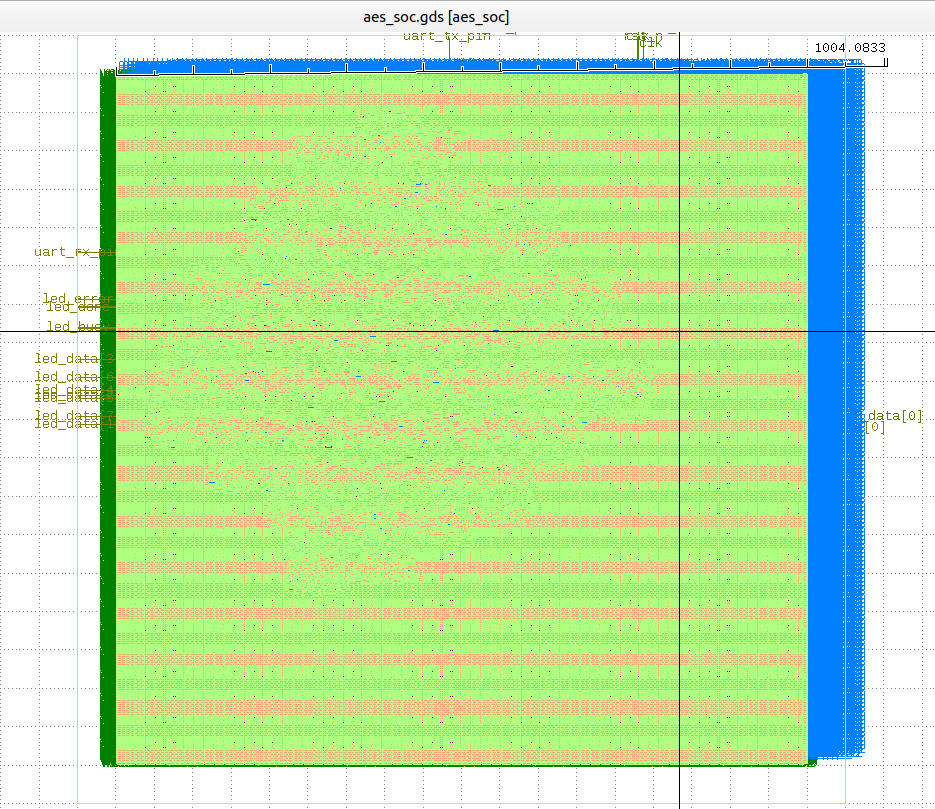
\includegraphics[width=\linewidth]{klayout_full_chip.png}}%
}

\begin{document}

\title{An Open-Source AES-128 Crypto Accelerator SoC with Design-for-Test:\\
RTL to Signoff-Clean GDSII in SkyWater~130\,nm}

% ---- BLIND: keep for camera-ready, comment out for double-blind review ----
\author{\IEEEauthorblockN{Akif Mohamed J\ \ and\ \ Nandikha M}
\IEEEauthorblockA{\textit{Department of Electronics and Communication Engineering} \\
\textit{Government College of Engineering, Srirangam, Tamil Nadu, India} \\
akifmohamed2217@gmail.com}}
% ---------------------------------------------------------------------------

\maketitle

\begin{abstract}
This paper presents an AES-128 encryption accelerator System-on-Chip (SoC)
carried from Verilog RTL to signoff-clean GDSII entirely with open-source
tools on the SkyWater 130\,nm PDK, with design-for-test (DFT) as a first-class
objective. An iterative ten-round datapath with on-the-fly key expansion is
integrated behind a UART command interface. Two flow configurations are
reported: a 67.6\% core-utilization baseline, and a DFT configuration in
which all 745 flip-flops are replaced by scan flip-flops (100\% sequential
scan coverage, zero RTL changes) by a custom OpenLane~2 step operating on the
synthesized netlist, alongside a March~C$^-$ memory BIST verified by fault
injection. Both configurations close timing at 50\,MHz with zero setup and
hold violations across nine corners, pass DRC with zero violations, and match
LVS exactly. Encryption latency of 10 cycles (200\,ns, 0.64\,Gbps) is
measured by an in-design cycle counter on an Artix-7 FPGA and independently
reproduced in simulation; four known-answer vectors, including the NIST
SP~800-38A and FIPS-197 Appendix~B references, pass with zero bit errors.
Post-layout power analysis on extracted parasitics yields 6.08\,mW at the
typical corner (0.122\,mW/MHz; 1.22\,nJ per block). All sources, scripts, and
run artifacts are released for reproduction.
\end{abstract}

\begin{IEEEkeywords}
AES-128, design-for-test, scan, memory BIST, SkyWater 130nm, OpenLane,
open-source EDA, physical design, GDSII, FPGA validation
\end{IEEEkeywords}

\section{Introduction}
The Advanced Encryption Standard (AES)~\cite{fips197} remains the workhorse of
symmetric cryptography in embedded and IoT systems. Two trends make an
open, fully documented ASIC implementation valuable today. First, hardware
accelerators dominate software on energy-constrained devices: the best
published bitsliced AES-128 on an ARM Cortex-M4 requires about 80
cycles/byte~\cite{kimseo25}, whereas the accelerator in this paper completes
a 128-bit block in 10 clock cycles. Second, the maturing of open-source EDA
flows~\cite{openlane,openroad,yosys} and the open SkyWater 130\,nm
PDK~\cite{sky130} have made full RTL-to-GDSII implementation accessible
outside industry; yet published cryptographic implementations that document
complete signoff, DFT structures, measured latency, and post-layout power
remain scarce.

Most published AES hardware stops at RTL simulation or FPGA prototyping;
open-source silicon efforts such as the multi-algorithm crypto accelerator
taped out through the Google/SkyWater shuttle program~\cite{singhali} report
no measured benchmark data and no DFT. This paper addresses that gap with a
complete, reproducible implementation whose distinguishing property is that
every reported number traces to a committed artifact.

\textbf{Contributions.}
\begin{enumerate}
\item A complete RTL-to-GDSII implementation of an AES-128 SoC in
SkyWater~130\,nm using OpenLane~2.3.10, with DRC-clean layout, exact LVS
match, and zero setup/hold violations across nine timing corners in two flow
configurations.
\item DFT insertion performed at the netlist level inside an open flow: a
custom OpenLane step maps all 745 flip-flops to scan flip-flops (100\%
sequential coverage, single clock domain) with no RTL modification, and a
March~C$^-$ memory BIST is verified by behavioral fault injection.
\item Multi-level validation: four known-answer vectors in simulation
including NIST SP~800-38A and FIPS-197 Appendix~B; on-FPGA measurement of the
200\,ns encryption latency on an Artix-7 FPGA; and disclosed post-layout
power analysis on extracted parasitics.
\item Documented negative results where tools fell short: scan-chain
stitching was attempted at two flow points and is characterized by its error
signature; a floorplan sizing pitfall (ignored absolute dimensions) and its
fix are reported for the community.
\end{enumerate}

\section{Background and Related Work}
AES-128 operates on 128-bit blocks under a 128-bit key through an initial
key addition and ten rounds of SubBytes, ShiftRows, MixColumns, and
AddRoundKey, with the final round omitting MixColumns~\cite{fips197,sp80038a}.
Hardware implementations span the design space from compact iterative cores
to unrolled pipelines: Satoh et al.\ established the classic area/throughput
trade-off~\cite{satoh01}; Mathew et al.\ demonstrated aggressive
low-voltage operation down to 340\,mV in 22\,nm tri-gate
CMOS~\cite{mathew15}; and Hammad et al.\
surveyed energy-efficient IoT implementations~\cite{hammad20}. On the
software side, Schwabe and Stoffelen reported 554.4 cycles/block for
table-based AES-128-CTR on Cortex-M4~\cite{schwabe17}, and fixslicing
currently holds the Cortex-M4 record near 80 cycles/byte~\cite{kimseo25},
while measured mbedTLS runs at 71 cycles/byte~\cite{mbedtlsbench}.

Table~\ref{tab:related} positions this work. No prior open AES SoC
publication combines (i) full physical signoff data, (ii) measured on-FPGA
latency, (iii) DFT evidence (BIST plus scan-cell mapping), and (iv)
post-layout power analysis.

\begin{table}[htbp]
\caption{Positioning relative to representative prior work}
\label{tab:related}
\centering
\footnotesize
\setlength{\tabcolsep}{3.5pt}
\begin{tabular}{lcccc}
\toprule
Work & Node & Signoff & DFT & Measured \\
\midrule
Satoh et al.~\cite{satoh01} & 0.11\,$\mu$m & \checkmark & -- & \checkmark \\
Mathew et al.~\cite{mathew15} & 22\,nm & \checkmark & -- & \checkmark \\
Hammad et al.~\cite{hammad20} & 180/65\,nm & partial & -- & \checkmark \\
Singhali~\cite{singhali} & sky130 & taped out & -- & -- \\
Software: fixslicing~\cite{kimseo25} & Cortex-M4 & n/a & n/a & 80 c/B \\
\textbf{This work} & \textbf{sky130} & \textbf{\checkmark} & \textbf{\checkmark} & \textbf{\checkmark} \\
\bottomrule
\end{tabular}
\end{table}

\section{SoC Architecture}

\begin{figure*}[!t]
\centering
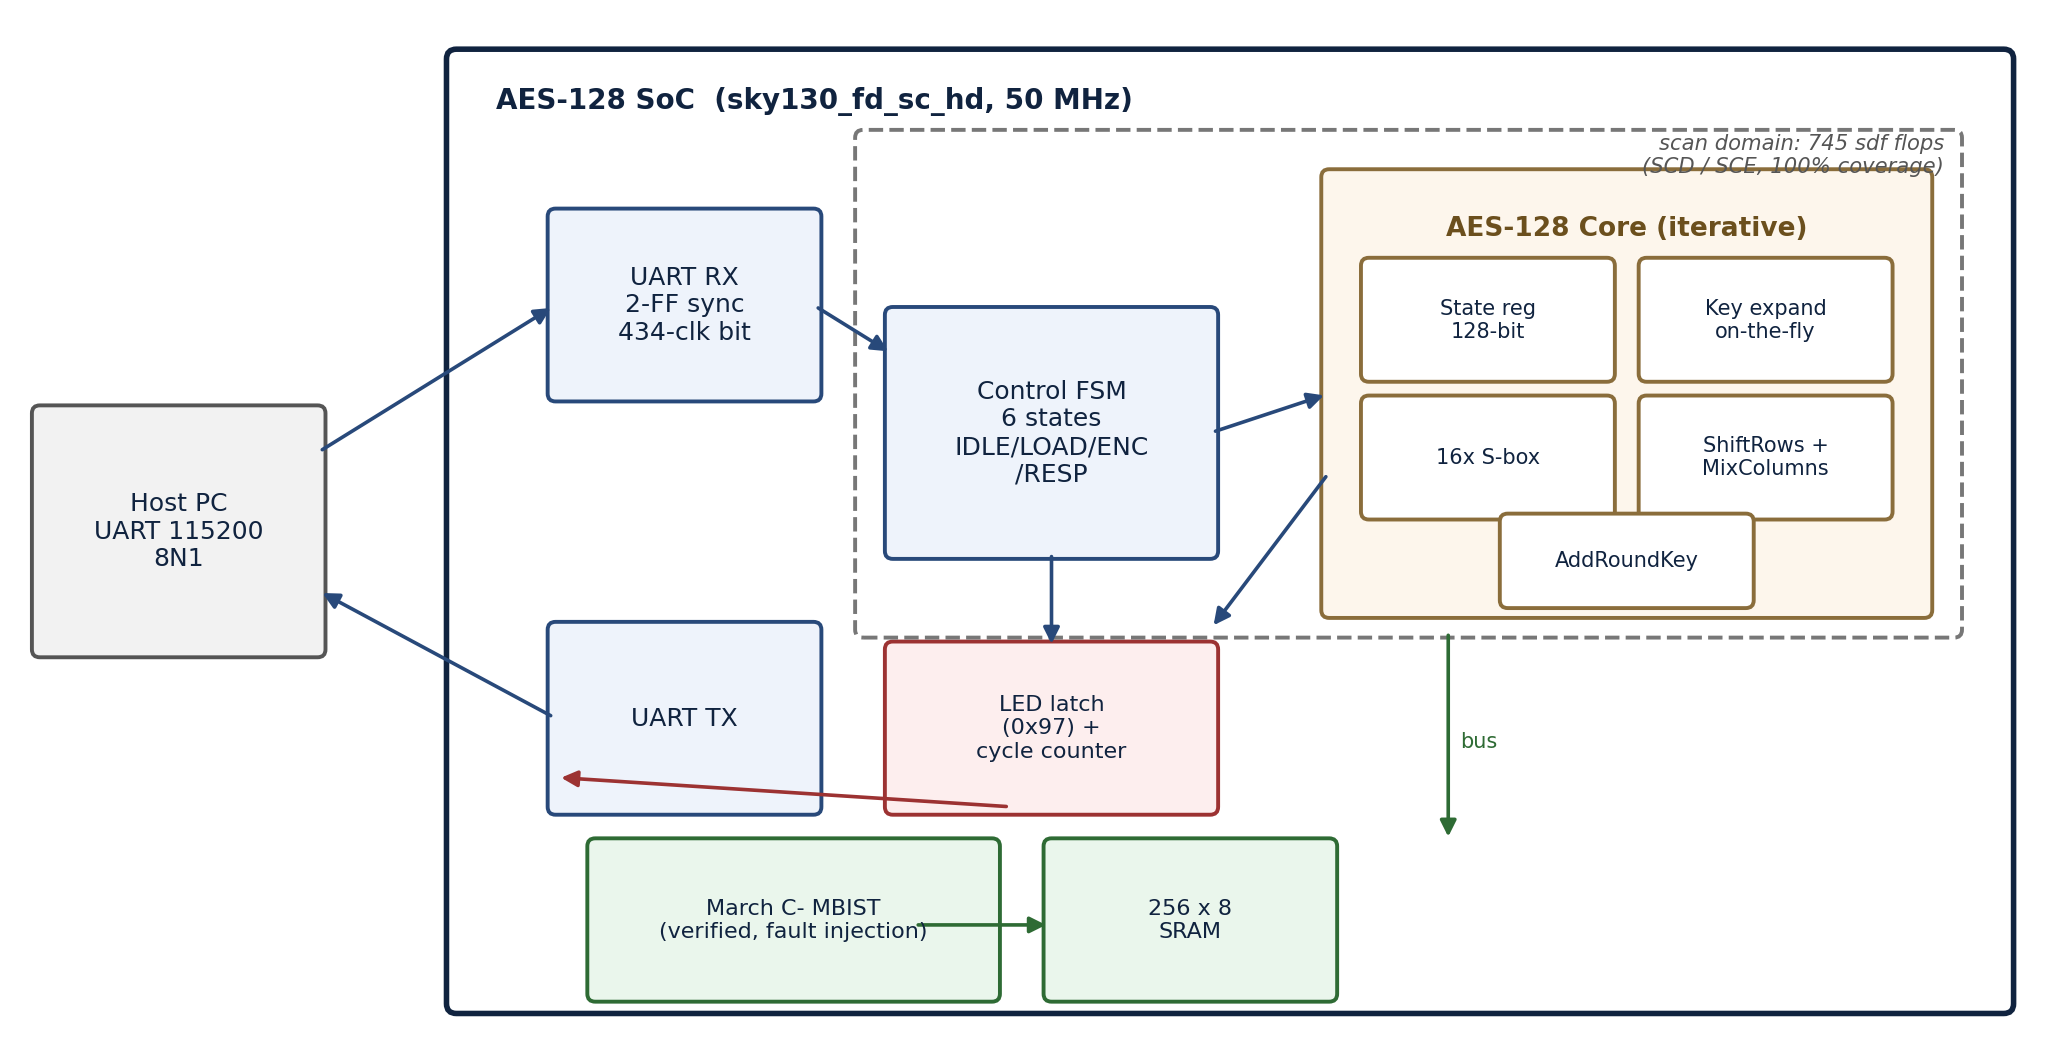
\includegraphics[width=0.95\textwidth]{soc_block.png}
\caption{SoC architecture. The iterative AES-128 core and the six-state
control FSM form a single-clock scan domain of 745 scan flip-flops (dashed
boundary, SCD/SCE pins); the March~C$^-$ MBIST verifies the
256$\times$8 SRAM independently of the scan domain.}
\label{fig:block}
\end{figure*}

\subsection{Iterative AES-128 Core}
The core implements one encryption round as combinational logic and reuses
it ten times under finite-state-machine control: a 128-bit state register;
sixteen parallel combinational S-boxes; wiring-only ShiftRows; GF($2^8$)
MixColumns over the AES irreducible polynomial; and an on-the-fly key
expansion unit, avoiding storage of eleven round keys. The interface is
\texttt{clk}, active-low \texttt{rst\_n}, \texttt{start}, 128-bit key and
plaintext, \texttt{ciphertext}, \texttt{done}, and \texttt{busy}. The busy
window is exactly ten cycles, consistent with the measured latency reported
in Section~\ref{sec:validation}.

\subsection{UART SoC Wrapper}
The core is wrapped in a minimal SoC with a 115200-baud 8N1 UART interface.
A command frame is 33 bytes: command byte \texttt{0xAE}, 16 key bytes, and
16 plaintext bytes, most-significant byte first. The response frame is 17
bytes: status \texttt{0xAA} followed by the 16 ciphertext bytes. The final
(least significant) ciphertext byte drives eight LEDs, giving a visible
known-answer check: 0x97 for the NIST SP~800-38A vector~1. A six-state Moore
FSM sequences idle, key load, plaintext load, encryption wait, status
transmit, and ciphertext transmit; a non-encrypt command byte asserts an
error flag by design. The UART receiver uses a two-flop synchronizer and a
434-clock-per-bit oversampling divider at 50\,MHz.

\section{Open-Source Physical Design Flow}
\label{sec:flow}
\subsection{Toolchain}
The flow is OpenLane~2.3.10 on Ubuntu~22.04: Yosys~0.46 synthesis, OpenROAD
(build \texttt{edf00dff}) for floorplanning through detailed routing, OpenSTA
for timing, Magic~8.3.489 for DRC and extraction, Netgen~1.5.278 for LVS, and
KLayout for streaming, targeting the sky130A PDK (volare version
\texttt{0fe599b2}) with the sky130\_fd\_sc\_hd cell library. All versions are
quoted from tool-log banners rather than assumed.

\subsection{Floorplan Sizing: A Documented Pitfall}
An early configuration specified absolute die and core rectangles; the flow
silently ignored them, fixing utilization at 20.2\%. Switching to relative
sizing (a core-utilization target with the flow computing dimensions)
produced the 67.6\% baseline configuration. Because this behavior differs
across OpenLane versions, we report it explicitly: absolute sizing keys may
be accepted but not honored, and utilization should be verified from
placement logs rather than assumed from configuration inputs.

\begin{figure}[!t]
\centering

\includegraphics[width=\linewidth]{klayout_std_cells.png}
\caption{Placement detail: sky130\_fd\_sc\_hd standard cells (KLayout view).}
\label{fig:stdcells}
\end{figure}

\subsection{DFT-Enabled Configuration}
Scan-cell replacement is performed by OpenROAD's \texttt{scan\_replace} on
the synthesized netlist, inserted into the flow as a custom step
(\texttt{AesDFT.ScanReplace}) immediately after synthesis and its checkers,
before power-connection setup and floorplanning. No RTL is modified at any
point. All 745 flip-flops map to scan flip-flops: 731
\texttt{sdfrtp\_2} (asynchronous reset) and 14 \texttt{sdfsbp\_2}
(asynchronous set, dual output) --- 100\% sequential coverage in a single
clock domain. Because scan cells are larger than their functional
counterparts, synthesized cell area grows 44\% (116.8k to 168.0\,$\mu$m$^2$
at the synthesis stage); the floorplan utilization target is compensated
(38\% pre-scan-equivalent) so that the placed design lands at a routable
51.9\%.

\begin{figure}[!t]
\centering
\LayoutFullChip
\caption{Full-chip layout view of the open-source flow implementation
(KLayout, committed GDSII of the repository).}
\label{fig:layout}
\end{figure}

\section{Design-for-Test Infrastructure}
\label{sec:dft}
\textbf{Memory BIST.} The 256$\times$8 SRAM is wrapped by a March~C$^-$
controller with a two-wait-state read pipeline matched to the memory's
registered output. Correctness is verified in simulation by behavioral
fault injection of both polarities: a fault-free memory passes, and an
injected stuck-at-0 at address 42, bit~0 is detected with the failing
address reported. This establishes that the BIST detects real defects, not
merely that it executes.

\textbf{Scan-cell mapping.} As described in Section~\ref{sec:flow}, the
complete sequential population (745/745) is replaced by scan-capable cells
inside the flow, yielding a scan-ready netlist and GDS with 100\% sequential
coverage.

\textbf{Chain stitching: attempted and characterized.} OpenROAD's
\texttt{insert\_dft} was invoked at two flow points: after detailed
placement, and again after post-CTS timing repair (i.e., with a synthesized
clock tree present). In both cases the command completes without error but
creates zero scan cells, emitting \texttt{DFT-0005} (``no valid clock
connected'') for every flip-flop; 745$\times$2 scan pins consequently remain
unconnected in the released GDS, which we disclose. The result is a
characterization of the available build: chain stitching with this OpenROAD
revision requires clock-domain resolution that the bundled \texttt{dft}
module does not provide for this design at either insertion point; the
scan-ready architecture is the contribution, and stitching with a newer
build is future work. Formal equivalence checking is likewise not applicable
to an unstitched scan netlist; equivalence is established by simulation
(Section~\ref{sec:validation}).

\section{Verification, Validation, and Power Analysis}
\label{sec:validation}
\subsection{Functional Verification}
RTL simulation on Icarus Verilog (versions 11.0 and 12.0) passes four
known-answer vectors: NIST SP~800-38A ECB-AES128 vector~1, FIPS-197
Appendix~B, an all-zero KAT, and an all-ones KAT, with zero bit errors. The
SoC-level testbench exercises the complete UART protocol---command decode,
33-byte frame reception, status and ciphertext transmission---and checks all
16 ciphertext bytes, the status byte, and the LED value. Two testbench
engineering points proved essential and are documented for reuse:
pulse-shaped signals (the 10-cycle busy window) must be captured by
background monitors rather than sequential waits, and a software UART
receiver must re-arm its start-bit edge sensitivity inside the transmitter's
bit period (this design uses 435-clock bits with a $\sim$2-clock inter-byte
gap), otherwise capture misframes deterministically.

\subsection{FPGA Hardware Validation}
\begin{figure}[!t]
\centering
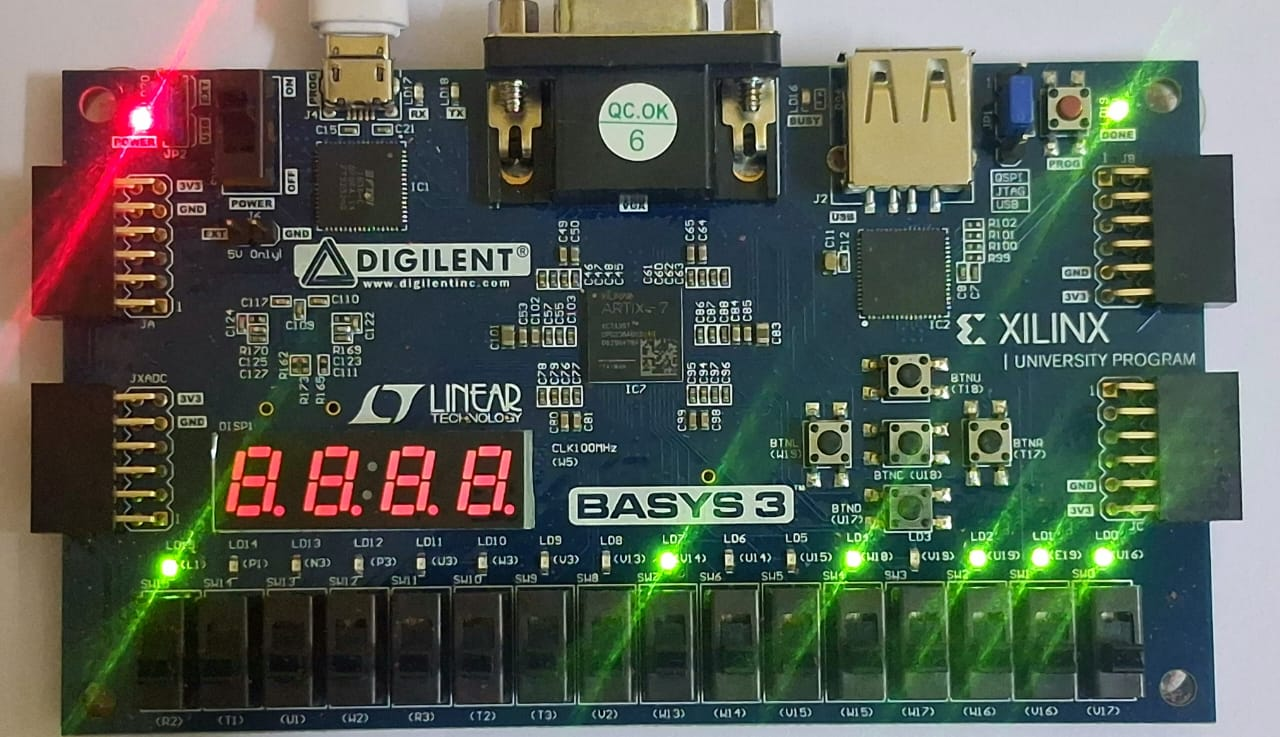
\includegraphics[width=\linewidth]{basys3_demo.jpg}
\caption{FPGA validation on a Digilent Basys3 (Artix-7 XC7A35T): LEDs
display 0x97, the final ciphertext byte of NIST SP~800-38A vector~1.}
\label{fig:fpga}
\end{figure}
The design runs on a Digilent Basys3 board (Artix-7 XC7A35T) under Vivado
2017.4 (WebPACK). A host script sends the SP~800-38A vector-1 frame over
USB-UART; the board returns status \texttt{0xAA} followed by the exact
16-byte NIST ciphertext, and the LEDs display 0x97. An in-design cycle counter
latches the busy window at exactly 10 cycles, i.e., 200\,ns at the 50\,MHz
board clock---agreeing with simulation and establishing the 0.64\,Gbps
throughput figure by measurement rather than estimation.

\begin{figure}[!t]
\centering
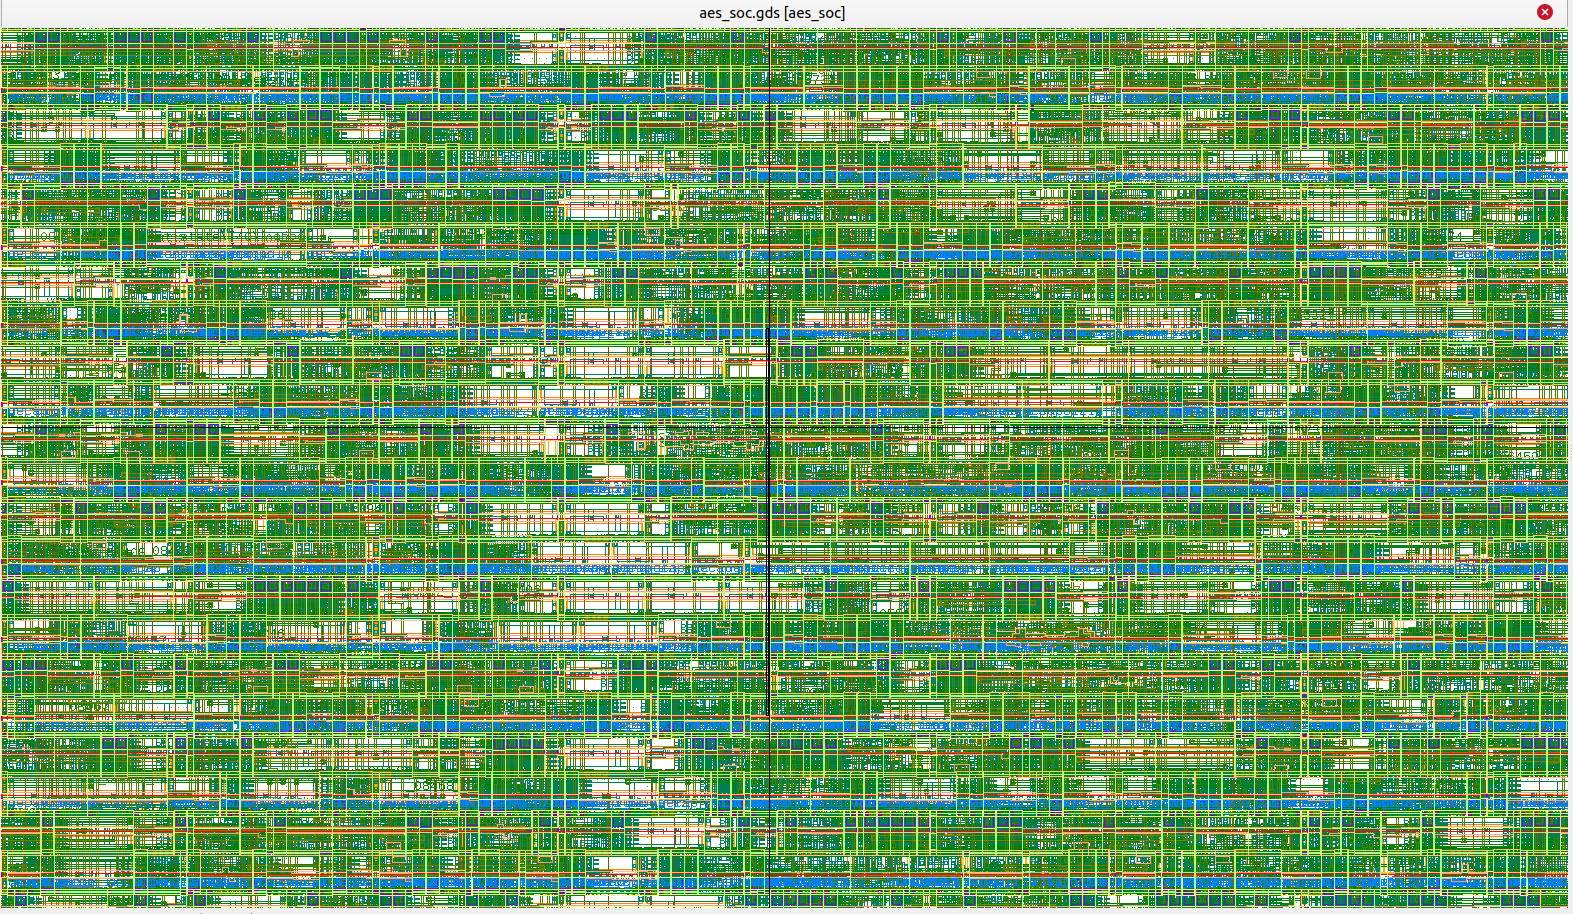
\includegraphics[width=\linewidth]{klayout_metal_routing.png}
\caption{Metal routing view over the core area (KLayout).}
\label{fig:routing}
\end{figure}

\subsection{Post-Layout Power Analysis}
Power is \emph{analyzed}, not silicon-measured, and the method is disclosed:
OpenSTA on the routed DEF with extracted SPEF parasitics, 50\,MHz clock,
switching activity 0.10, duty 0.5. Table~\ref{tab:power} reports all three
corners. The group split is 39\% sequential, 29\% combinational, and 31\%
clock, and the typical-corner total corresponds to 0.122\,mW/MHz and
1.22\,nJ per 128-bit block.

\begin{table}[htbp]
\caption{Post-layout power analysis (activity 0.10, duty 0.5, 50\,MHz)}
\label{tab:power}
\centering
\footnotesize
\setlength{\tabcolsep}{4.0pt}
\begin{tabular}{lcccc}
\toprule
Corner & Internal & Switching & Leakage & Total \\
\midrule
tt (25\,C, 1.80\,V) & 3.58\,mW & 2.50\,mW & 0.05\,$\mu$W & 6.08\,mW \\
ss (100\,C, 1.60\,V) & 2.91\,mW & 1.97\,mW & 55.7\,$\mu$W & 4.94\,mW \\
ff ($-$40\,C, 1.95\,V) & 4.07\,mW & 2.93\,mW & 0.09\,$\mu$W & 7.00\,mW \\
\bottomrule
\end{tabular}
\end{table}

\section{Results and Comparison}
\label{sec:results}
Table~\ref{tab:summary} summarizes both flow configurations; both completed
all flow stages to GDSII. Detailed routing converges to zero violations in
seven iterations (16062$\to$9323$\to$8993$\to$1312$\to$80$\to$13$\to$0);
total wirelength is 560{,}956\,$\mu$m; worst IR drop is 0.021\%. Nine
timing corners report zero setup and hold violations in both runs.

Against software, the measured 10-cycle block latency compares with 1136
cycles/block for measured mbedTLS AES-128 on Cortex-M4 (71
cycles/byte~\cite{mbedtlsbench}) --- a 114$\times$ cycle-count reduction ---
and with about 1280 cycles/block for the fastest published bitsliced
implementation~\cite{kimseo25} --- 128$\times$. At equal clock frequency the
throughput advantage is of the same order, versus a software baseline that
itself outperforms classic table-based code by roughly
2.3$\times$~\cite{schwabe17}.

\begin{table}[htbp]
\caption{Implementation summary (all values from run artifacts)}
\label{tab:summary}
\centering
\footnotesize
\setlength{\tabcolsep}{3.0pt}
\begin{tabular}{lcc}
\toprule
 & Baseline & DFT-enabled \\
\midrule
Die / core ($\mu$m$^2$) & 240k / 224k & 326k / 308k \\
Core utilization & 67.6\% & 51.9\% \\
Sequential elements & 745 & 745 (100\% scan) \\
Setup slack (worst/tt) & --- / +14.07\,ns & +7.22 / +14.06\,ns \\
Hold slack (worst) & +0.29\,ns & +0.107\,ns \\
Timing violations (9 corners) & 0 & 0 \\
DRC (Magic / KLayout) & 0 / 0 & 0 / 0 \\
LVS & match & match \\
Antenna residuals & 2 marginal & 1 net + 1 pin \\
MBIST & \multicolumn{2}{c}{March C$^-$, fault-inj.\ verified} \\
Latency @ 50\,MHz & \multicolumn{2}{c}{10 cycles = 200\,ns (FPGA)} \\
Throughput & \multicolumn{2}{c}{0.64\,Gbps} \\
Power (tt, analysis) & --- & 6.08\,mW / 0.122\,mW/MHz \\
\bottomrule
\end{tabular}
\end{table}

\section{Limitations and Future Work}
We state limitations explicitly. (i) The GDS is not fabricated: all physical
results are signoff analyses; the FPGA measurement validates function and
latency, not silicon power or yield. (ii) Power figures are analyses under a
disclosed default activity, not measurements. (iii) Scan chains are mapped
but not stitched, as characterized in Section~\ref{sec:dft}; 109 nets also
lack RC annotation in extraction. (iv) Encryption only: decryption and
AES-192/256 are future work. Planned next steps: chain stitching with a
newer OpenROAD build; activity-annotated power from gate-level simulation;
DPA countermeasures; and silicon measurement through an open-shuttle
program.

\section{Conclusion}
An AES-128 SoC has been implemented from RTL to signoff-clean GDSII in
SkyWater 130\,nm with fully open tools, with DFT integrated at the netlist
level: 100\% scan-cell mapping of all 745 flip-flops via a custom flow step,
and a fault-injection-verified March~C$^-$ MBIST. The 200\,ns measured
latency, nine-corner clean timing, zero DRC violations, exact LVS match, and
disclosed power analysis---each traceable to a committed artifact---provide
a reproducible reference point for open-source cryptographic silicon.

% Acknowledgment: omitted at submission; re-add at camera-ready if desired.

\begin{thebibliography}{00}
\bibitem{fips197} National Institute of Standards and Technology,
``Advanced Encryption Standard (AES),'' FIPS Publication 197, Nov. 2001.
\bibitem{sp80038a} NIST, ``Recommendation for Block Cipher Modes of
Operation,'' SP 800-38A, 2001.
\bibitem{satoh01} A. Satoh, S. Morioka, K. Takano, and S. Munetoh, ``A
compact Rijndael hardware architecture with S-box optimization,'' in
\emph{Proc. ASIACRYPT}, 2001, pp. 239--254.
\bibitem{mathew15} S. K. Mathew et al., ``340\,mV--1.1\,V, 289\,Gbps/W,
2090-gate NanoAES hardware accelerator with area-optimized encrypt/decrypt
GF($2^4$)$^2$ polynomials in 22\,nm tri-gate CMOS,'' \emph{IEEE J. Solid-State
Circuits}, vol. 50, no. 4, pp. 1048--1058, Apr. 2015.
\bibitem{hammad20} H. Hammad, S. Tatapudi, R. Adegbija, and T. Mohsenin,
``Energy-efficient AES implementations for IoT devices,'' in \emph{Proc.
GLSVLSI}, 2020, pp. 187--192.
\bibitem{schwabe17} P. Schwabe and K. Stoffelen, ``All the AES you need on
Cortex-M3 and M4,'' in \emph{Proc. CHES}, 2017, pp. 180--194.
\bibitem{kimseo25} H. Kim and H. Seo, ``Optimizing AES-GCM on 32-bit ARM
Cortex-M4 microcontrollers: Fixslicing and FACE-based approach,'' \emph{ACM
Trans. Embedded Comput. Syst.}, vol. 24, no. 6, pp. 1--24, 2025,
doi:10.1145/3766074.
\bibitem{mbedtlsbench} Mozilla SensorWeb Project, ``mbed TLS benchmark
(NUCLEO-446RE, Cortex-M4),'' GitHub wiki, 2016.
[Online]. Available: https://github.com/mozilla-sensorweb/sensorweb-wiki
\bibitem{singhali} A. Singhali, ``Crypto accelerator chip (AES-128/256,
SHA-256) in SkyWater 130nm,'' GitHub repository, 2020. [Online]. Available:
https://github.com/asinghani/crypto-accelerator-chip
\bibitem{openlane} Efabless Corp., ``OpenLane 2 documentation,''
2024. [Online]. Available: https://openlane2.readthedocs.io
\bibitem{openroad} The OpenROAD Project, ``OpenROAD: unified physical design
implementation.'' [Online]. Available: https://theopenroadproject.org
\bibitem{yosys} C. Wolf, ``Yosys open synthesis suite.''
[Online]. Available: http://www.clifford.at/yosys/
\bibitem{sky130} Google and SkyWater Technology, ``SkyWater PDK 130nm
open-source process design kit.'' [Online]. Available:
https://github.com/google/skywater-pdk
\end{thebibliography}

\end{document}
